% some-then-none involving wrr in ALG_ID algorithm
\documentclass{standalone}

\usepackage{tikz}

\tikzset{wop/.style = {blue, very thick},
  rop/.style = {brown, very thick}}

% interval for operations
\newcommand{\itv}[5]{ % #1: start point; #2: end point; #3: operation name; #4: style; #name
  \coordinate (start #3) at #1;	% start point
  \coordinate (end #3) at #2;	% end point

  \draw[#4, |-|] (start #3) -- (end #3) % draw the interval
  node[pos = 0.5, above = 1mm, font = \Large] (#5) {\textsl{#3}}; % attach the operation name
}

\begin{document}
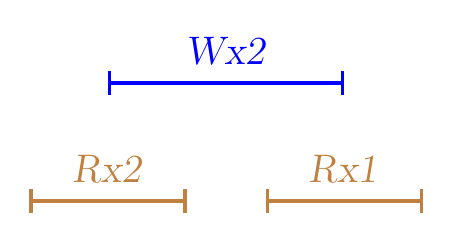
\begin{tikzpicture}
  \itv{(0,0)}{(2,0)}{Rx2}{rop}{rx2}
  \itv{(3,0)}{(5,0)}{Rx1}{rop}{rx1}

  \itv{(1,1.5)}{(4,1.5)}{Wx2}{wop}{wx2}
\end{tikzpicture}
\end{document}

